Descrição da interface de criação de cenários e alguns exemplos do que pode ser criado com ele.


\begin{figure}
	\centering
	\caption{Cenário 1}
	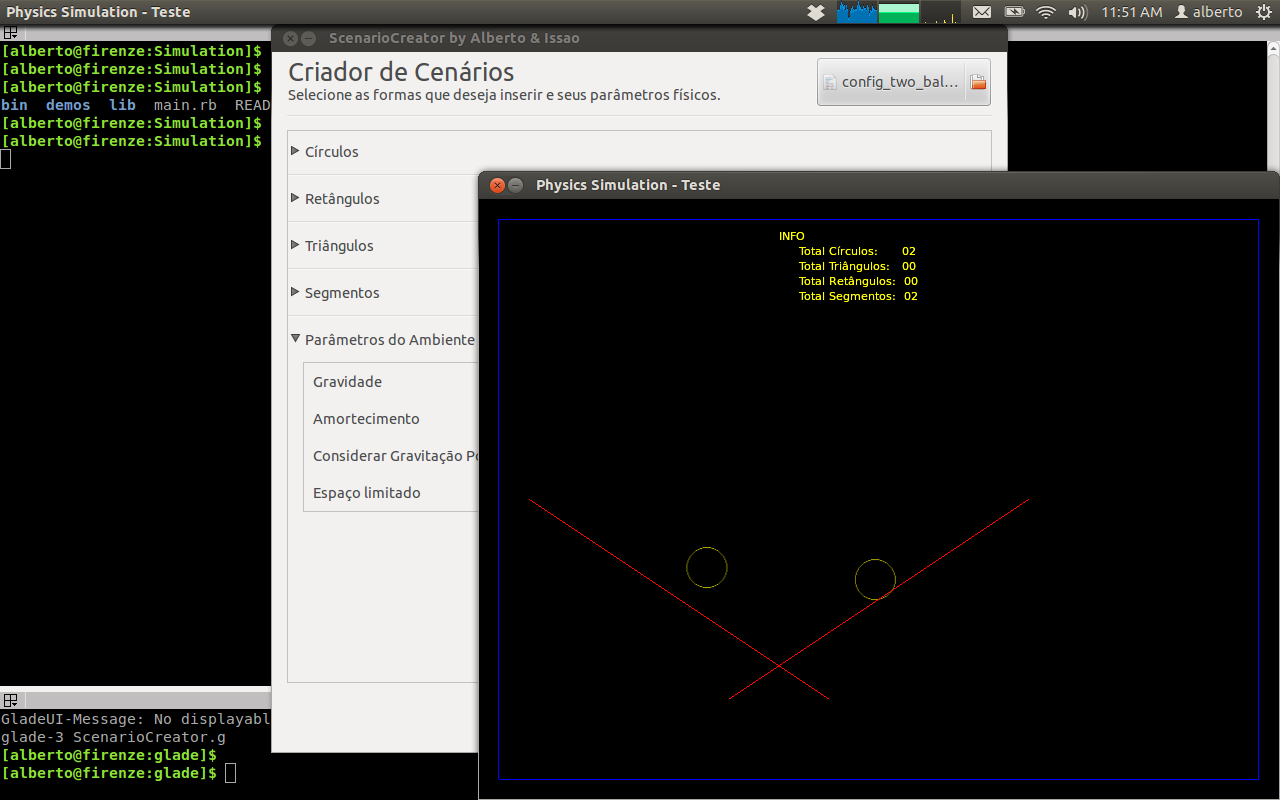
\includegraphics[scale=0.3]{images/cenario-two-balls.png}
	\hspace{0.5cm}
\end{figure}

  \begin{figure}
	\centering
	\caption{Cenario 2}
    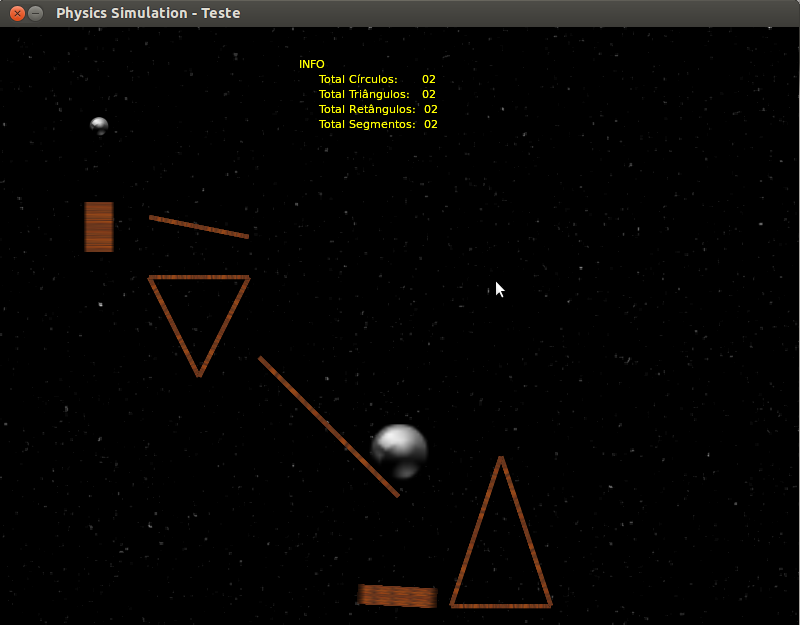
\includegraphics[scale=0.4]{images/cenario-todos.png}
    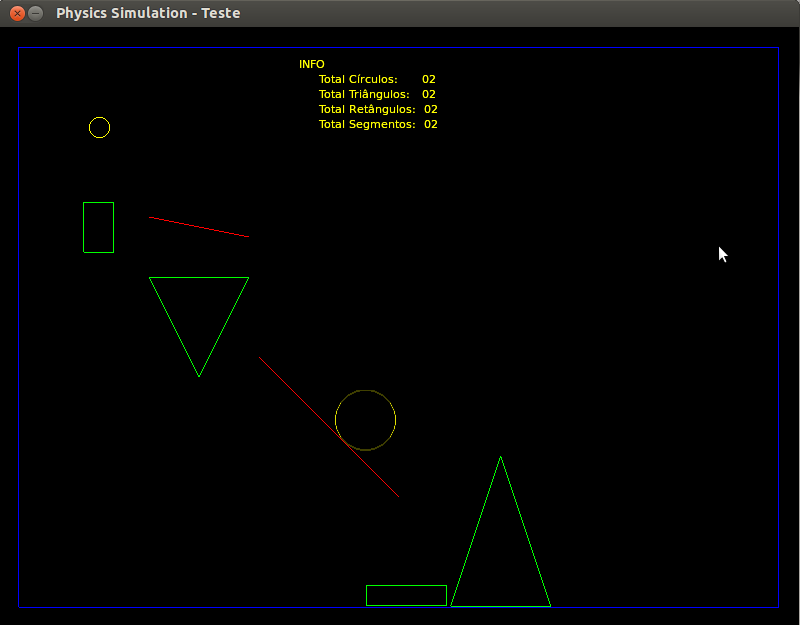
\includegraphics[scale=0.4]{images/cenario-todosE.png}
  \end{figure}

  \begin{figure}
	\centering
	\caption{Cenário Gravitacão 1}
    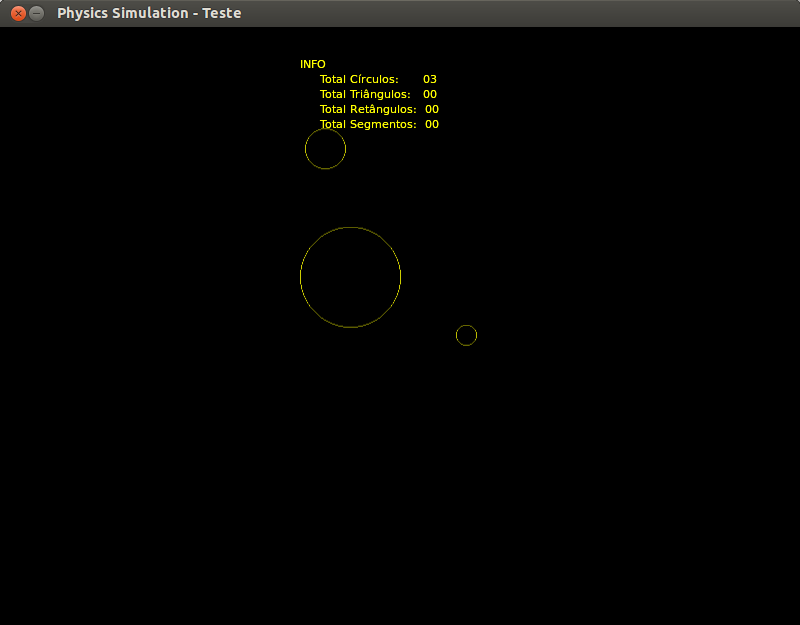
\includegraphics[scale=0.4]{images/cenario-gravitacao.png}
    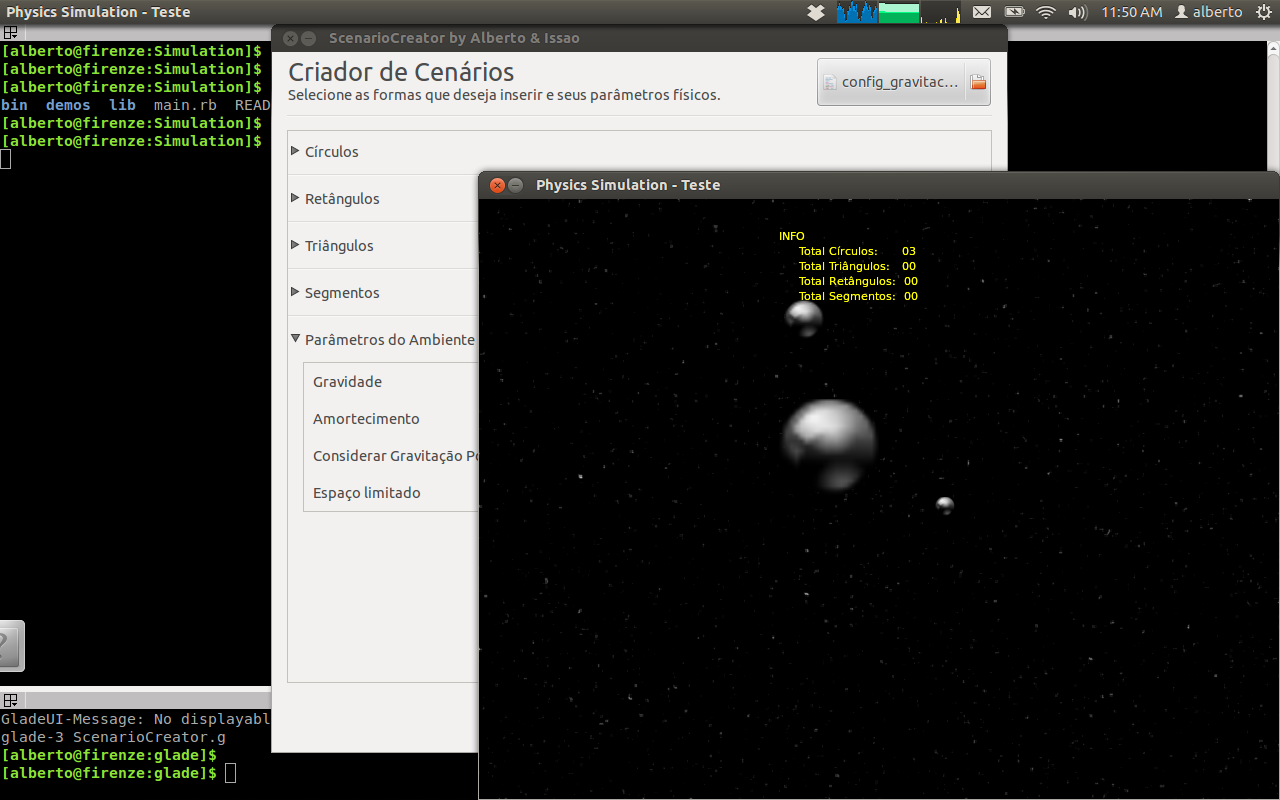
\includegraphics[scale=0.4]{images/cenario-gravitacao-2.png}
  \end{figure}

  \begin{figure}
	\centering
	\caption{Cenário Gravitacão 2}
    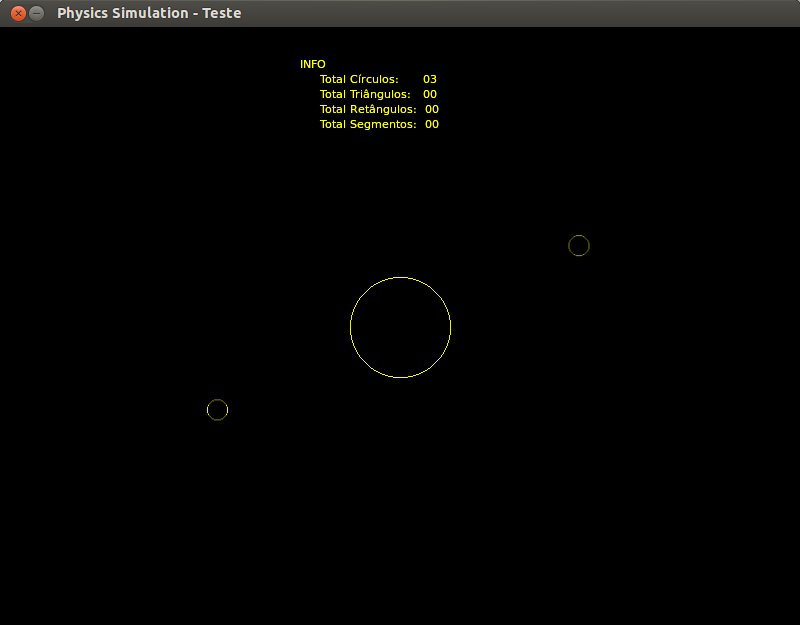
\includegraphics[scale=0.4]{images/cenario-gravitacao-3.png}
    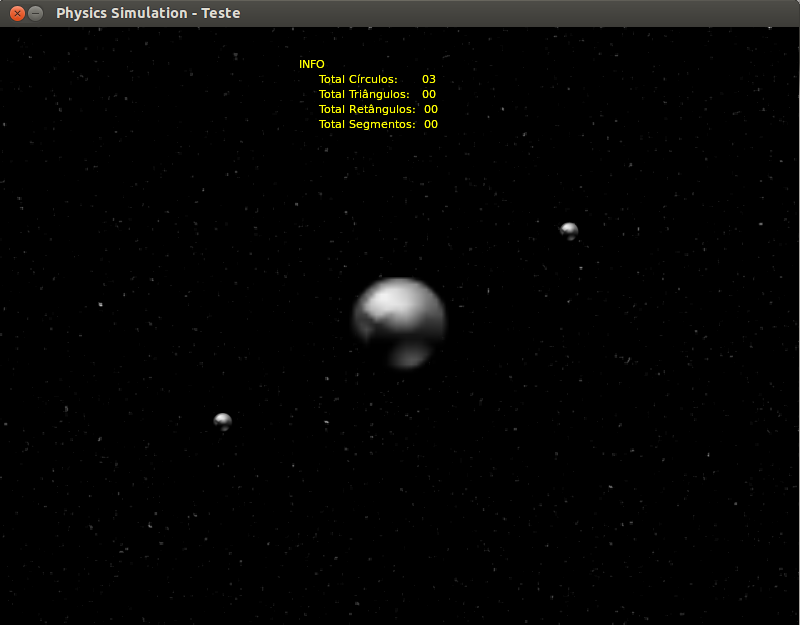
\includegraphics[scale=0.4]{images/cenario-gravitacao-4.png}
  \end{figure}

